\documentclass{article}

\PassOptionsToPackage{numbers,sort&compress}{natbib}
\usepackage[dblblindworkshop]{neurips_2026}
\workshoptitle{Trustworthy AI for Good Workshop}

\usepackage[utf8]{inputenc}
\usepackage[T1]{fontenc}
\usepackage{amsmath,amssymb,amsfonts,mathtools}
\usepackage{booktabs,tabularx,longtable,array,multirow}
\usepackage{graphicx}
\usepackage{xcolor}
\usepackage{microtype}
\usepackage{nicefrac}
\usepackage{url}
\usepackage{hyperref}
\usepackage[nameinlink,capitalise,noabbrev]{cleveref}
\usepackage{enumitem}

\definecolor{qnavy}{HTML}{17324D}
\definecolor{qgreen}{HTML}{2A9D78}
\definecolor{qorange}{HTML}{E28E2C}
\hypersetup{colorlinks=true,citecolor=qnavy,linkcolor=qnavy,urlcolor=qgreen}
\newcolumntype{Y}{>{\raggedright\arraybackslash}X}
\newcommand{\ind}{\mathbb{I}}
\newcommand{\Hmode}{\mathrm{H}}
\newcommand{\Amode}{\mathrm{A}}
\newcommand{\Cmode}{\mathrm{C}}
\newcommand{\UWCQ}{\textsc{U--W--C--Q}}
\newcommand{\Repo}{anonymous supplementary artifact}

\title{Q-OPS: A Reproducible Evidence Audit of Quantum Sampling for Trustworthy Human--AI Mode Allocation}
\author{Anonymous authors}

\begin{document}
\maketitle

\begin{abstract}
Organizations allocating work among humans, AI, and human--AI collaboration face accountability, reliability, review-capacity, exposure, and workflow-complementarity constraints. We formulate this as a synthetic governance-constrained benchmark and audit quantum sampling only inside a four-task retained set derived from strong classical controls. The \UWCQ{} stack combines uniform feasible sampling (U), an incumbent-derived warm state (W), greedy/cluster-repair controls plus a classical certificate (C), and feasible-subspace statevector QAOA (Q). A frozen 32-instance evaluation yields strict feasible retained sets on 30/32 cases and cluster-repair gains on 25/32. At $p=2$, mean optimum mass rises from .0223 under uniform sampling to .1522 (paired difference .1299, 95\% bootstrap CI [.0991,.1640]); the matched 128-draw first-hit proxy falls from 36.50 to 12.94 draws. Yet only 9/32 cases pass a \emph{post-simulation} evidence gate, $p=1$ exceeds $p=2$ on 28/32 under unequal parameter searches, and composite feasibility holds for 27/32 incumbents despite zero explicit disallowed-mode violations. Thus the evidence is conditional noiseless probability concentration---not QPU, runtime, scaling, workplace-safety, or universal quantum advantage. The result is an auditable benchmark foundation and a falsifiable agenda for selective quantum adoption in human--AI organizations.
\end{abstract}

\section{Introduction}
\label{sec:introduction}

Future service organizations allocate work among humans, AI systems, and human--AI teams. Each choice changes expected service, cost, capacity, accountability, review burden, and exposure to correlated AI failures. Human--AI staffing is therefore an economic resource-allocation problem with hard operational and institutional constraints, not merely a scheduling toy. Research on human--AI interaction calls for explicit authority and oversight boundaries~\citep{amershi2019humanai,seeber2020machines}; service operations supplies capacity and reliability models~\citep{gans2003callcenters}; and sociotechnical analysis cautions that efficiency or a compact fairness proxy cannot stand in for stakeholder welfare~\citep{selbst2019fairness}.

Quantum optimization introduces a second adoption decision. Even if a statevector experiment concentrates probability on good candidates, using the quantum component may be irrational once classical alternatives, validation, delay, review, and risk costs are counted. Small noiseless demonstrations also do not establish QPU performance, wall-clock advantage, or scaling~\citep{preskill2018nisq,cerezo2021variational,bharti2022nisq}. Rigorous optimization benchmarks consequently emphasize standardized instances, strong counterfactuals, solution quality, resources, and reproducibility~\citep{koch2026qoblib}; application-centric frameworks additionally ask whether the complete workflow improves a meaningful task~\citep{finzgar2022quark}.

Q-OPS moves the question one level upward: \emph{when is there enough evidence to invoke quantum computation at all?} The architecture in \cref{fig:architecture} treats quantum computation as an optional expert after a strong classical stage and before an independent certificate and fallback. It distinguishes system-level benchmarking (a fixed stack), algorithm-level benchmarking (controlled solver comparison), and application-level benchmarking (incremental decision value for the same organizational problem). The frozen study reaches the second level only on selectively retained cores inside an application-oriented architecture.

\begin{figure*}[t]
\centering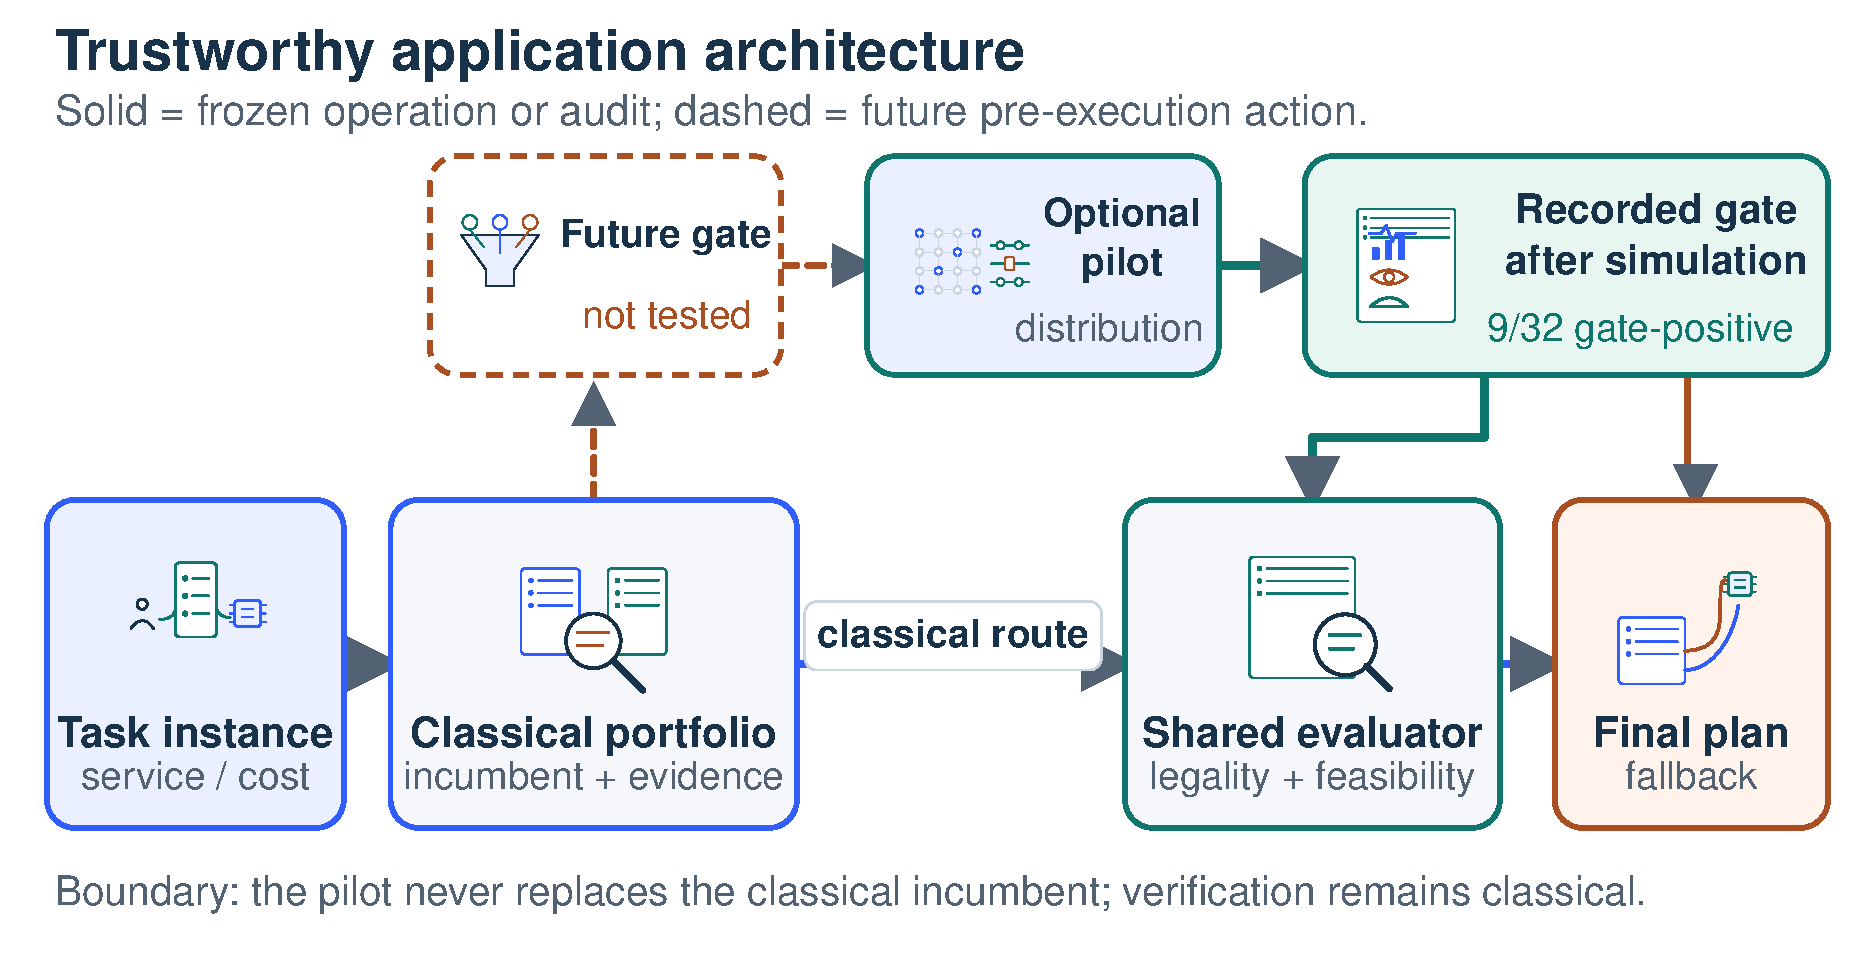
\includegraphics[width=\textwidth]{figs/fig1_architecture.pdf}
\caption{\textbf{Trustworthy application-level architecture.} Strong classical alternatives precede the recorded evidence gate; the quantum branch is optional; a shared classical evaluator and fallback bound operational acceptance. Dashed abstention/review is conceptual and was not evaluated. Clip art is semantic only; labels, arrows, gates, and evidence states are editable vector layers.}\label{fig:architecture}
\end{figure*}


The paper is organized around exactly three research-question--contribution pairs:
\begin{enumerate}[leftmargin=*,label=\textbf{RQ\arabic*.},itemsep=1pt,topsep=3pt]
\item \textbf{How can Human--AI staffing jointly represent service, cost, review scarcity, collaboration, correlated failures, and hard requirements?} We contribute a synthetic, governance-constrained benchmark with human-only, AI-only, and collaborative modes, empirical chance constraints, disruption scenarios, and an explicit composite feasibility predicate.
\item \textbf{When should a trustworthy decision system remain classical or run a quantum pilot?} We contribute an evidence-aware routing architecture driven by a multidimensional instance state, remaining classical headroom, ambiguity, feasibility, certification, and fallback. Abstention and human review are architectural actions, not evaluated policies in the frozen experiment.
\item \textbf{What conditional value survives strong counterfactuals and application-aware evidence boundaries?} We contribute a frozen, null-inclusive evaluation with matched sampling budgets, negative development stages, exact shared-field reproduction, and an evidence ladder that separates sampling improvement from optimization, application, and welfare claims.
\end{enumerate}

The headline result is deliberately two-sided. Nine of 32 held-out instances (28.13\%) satisfy the recorded post-simulation gate; across all 32 retained-core comparisons, $p=2$ statevector sampling has a 6.831$\times$ ratio of mean optimum probability over uniform feasible sampling. Independent evaluation records zero disallowed-mode violations, but composite feasibility holds for only 27/32 classical incumbents. The gate uses an observed quantum statistic and is not a prospective cost-saving router; $p=1$ exceeds $p=2$ on 28/32 cases under unequal search budgets; and stronger full-problem classical or hardware comparisons remain absent. A trustworthy system should maximize \emph{justified}, not maximal, quantum use.

\section{Established components and the integration gap}
\label{sec:related}

\paragraph{Quantum optimization.}
QAOA alternates cost and mixer evolutions to produce a parameterized distribution over combinatorial states~\citep{farhi2014qaoa,zhou2020qaoa}; reviews document many encodings, mixers and optimizers~\citep{blekos2024review,sawaya2023mixers}. The alternating-operator formulation makes constraint-preserving mixers explicit~\citep{hadfield2019alternating}, while warm-start QAOA uses classical information in initialization~\citep{egger2021warm}. Quantum scheduling is likewise an existing research area rather than a novelty of this work~\citep{werner2026scheduling}. Recent Nature reviews map the reverse interface---AI for quantum computing and quantum-system characterization~\citep{artificialintelligence2025quantum,mehta2026representing}; our study instead audits quantum sampling inside an AI-governance allocation problem. We contribute neither a new circuit family nor a claim that deeper QAOA must perform better.

\paragraph{Organizations, uncertainty and governance.}
Chance-constrained programming formalizes tolerance to stochastic constraint failure~\citep{charnes1959chance}, while service-operations research studies staffing and capacity under uncertain demand~\citep{gans2003callcenters}. Human--AI work adds authority, complementarity and coordination questions~\citep{amershi2019humanai,seeber2020machines,fuegener2026complementarity}. Algorithmic work assignment can also affect perceived fairness and productivity~\citep{bai2022algorithmic}; consequently, our regional AI-use dispersion is labeled an \emph{exposure regularizer}, not a validated fairness metric~\citep{selbst2019fairness,mehrabi2021fairness}. NIST and ISO governance frameworks motivate documented risks, measurement and human accountability~\citep{nist2023airmf,iso42001,iso23894}, but do not certify our synthetic benchmark.

\paragraph{Selection, abstention and reproducibility.}
Selective classification and learning-to-defer ask a model to abstain or hand off under uncertainty~\citep{geifman2017selective,madras2018defer}; classical algorithm selection asks which solver fits an instance~\citep{rice1976algorithm,kotthoff2014algorithm}. Our frozen gate is related in spirit but materially weaker: because it uses QAOA optimum mass, it partitions evidence \emph{after} simulation and cannot save quantum computation. Null-inclusive locked evaluation follows reproducibility norms that emphasize complete protocols and inspectable artifacts~\citep{pineau2021reproducibility}.

\begin{figure}[t]
  \centering
  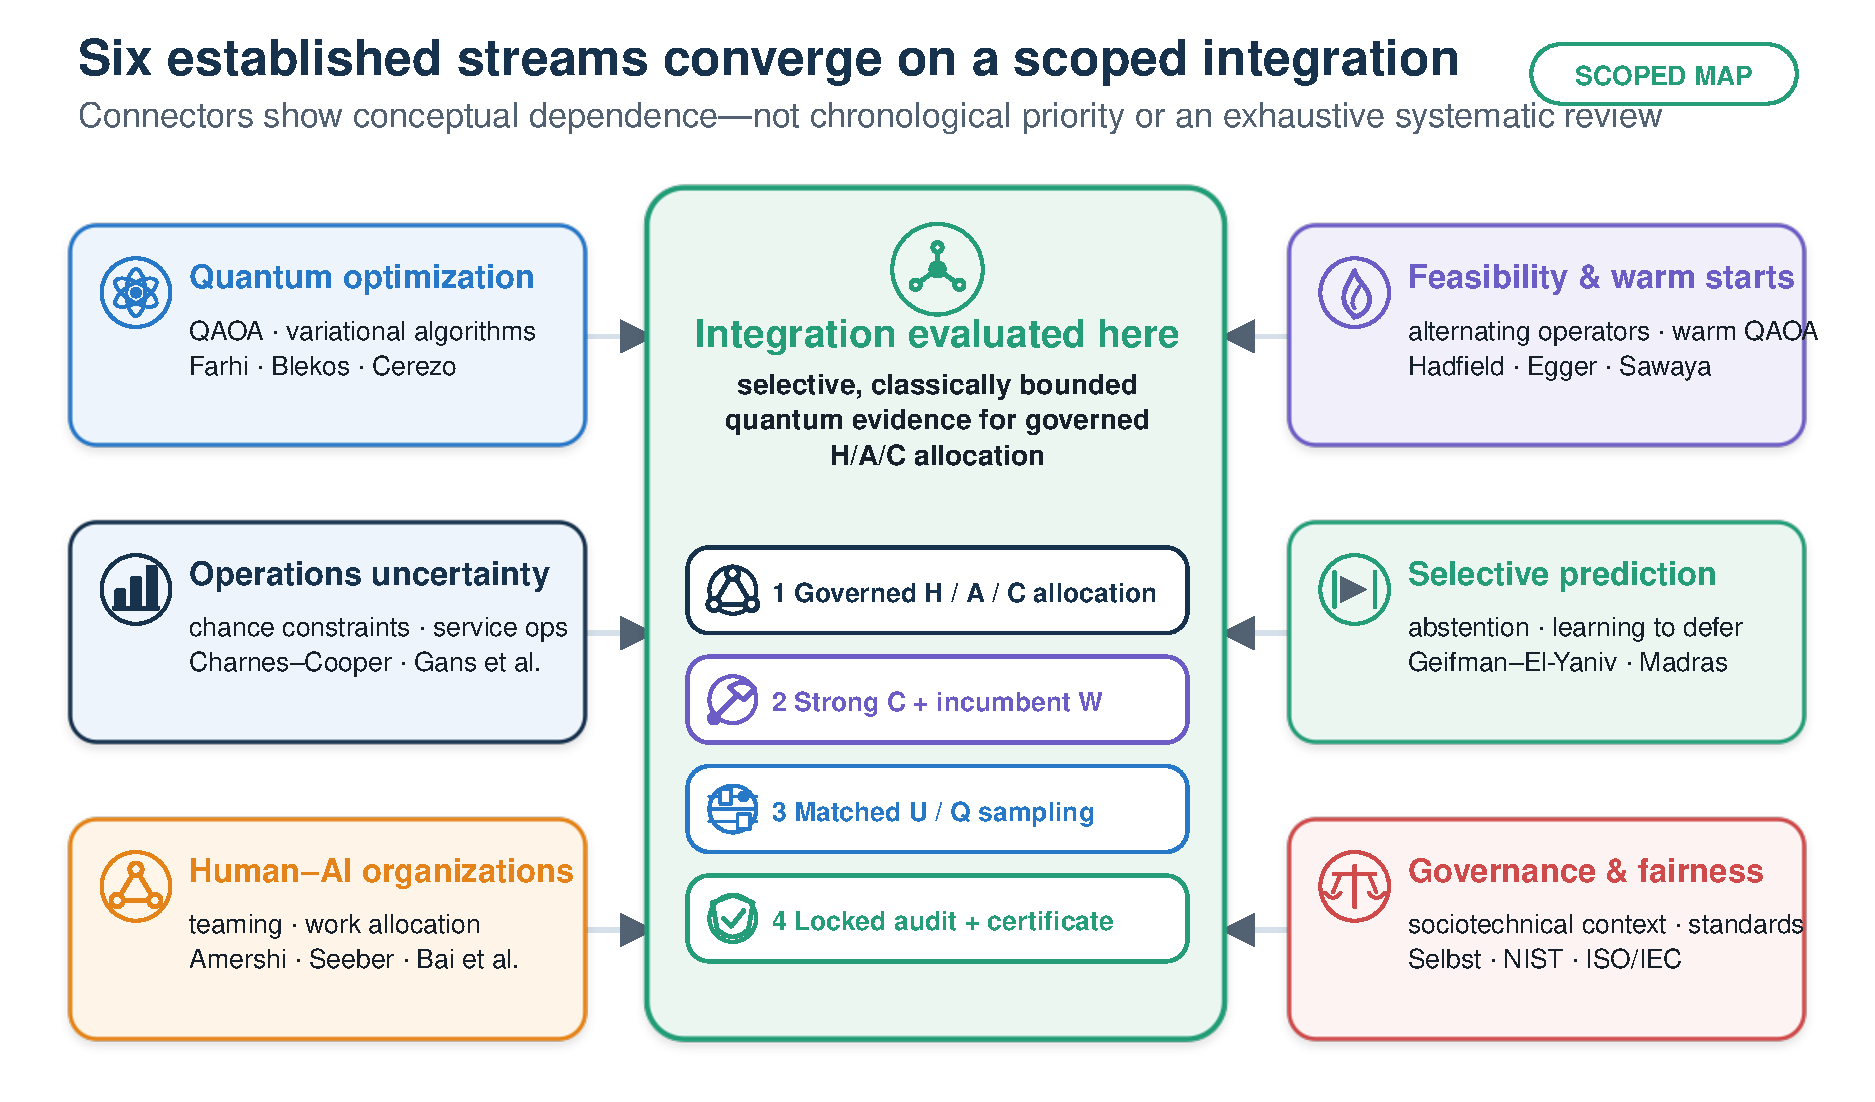
\includegraphics[width=\linewidth]{figs/fig4_literature_map.pdf}
  \caption{Scoped relationship map. Six established streams connect to the four-layer integration evaluated here: governed H/A/C allocation, strong classical structure and warm initialization, matched retained-set sampling, and locked classical certification. The short solid connectors encode conceptual dependence; the map is not a systematic-review flowchart or an exhaustive priority claim.}
  \label{fig:literature}
\end{figure}


\Cref{fig:literature} makes the novelty boundary visible. Each component is established. The gap addressed here is an auditable combination in which quantum sampling is conditioned on a governance-rich H/A/C evaluator, compared against strong classical structure, evaluated on held-out frozen instances, and bounded by a classical certificate. A systematic review could strengthen or refute this scoped integration claim; we do not infer ``first ever'' from the map.

\section{Governance-constrained H/A/C benchmark}
\label{sec:benchmark}

Let tasks $i\in I$ have duration $d_i$, priority $p_i$, value $v_i$, region $r(i)$ and an allowed mode domain $D_i\subseteq\{\Hmode,\Amode,\Cmode\}$. Human-mandatory tasks exclude $\Amode$. The assignment and explicit mode-violation count are
\begin{equation}
 y_i\in D_i,\qquad H(y)=\sum_{i\in I}\ind[y_i\notin D_i].
 \label{eq:mode}
\end{equation}
Costs are $C(y)=\sum_i d_i c_{i,y_i}$. Review-required AI-only tasks contribute one unit and collaborative tasks one quarter,
$R(y)=\sum_i r_i(\ind[y_i=\Amode]+.25\ind[y_i=\Cmode])$, with overflow $R_+(y)=[R(y)-B_R]_+$.

Tasks form workflow clusters $k$. Writing $n_k^C$ for the collaboration count, $h_k$ for its threshold and $m_k$ for the number of distinct modes, the cluster term is
\begin{equation}
 G(y)=\sum_k\!\left(B_k\ind[n_k^C\ge h_k]-A_k\ind[\forall i\!\in\!k:y_i=\Amode]-J_k(m_k-1)_+\right).
 \label{eq:cluster}
\end{equation}
This distinguishes workflow complementarity from an assumption that every individual collaborative assignment is beneficial. A coded exposure term $P_{\rm exp}(y)=2\operatorname{sd}_{r}(a_r)$ penalizes dispersion in regional AI-only rates $a_r$. It is a transparent benchmark regularizer, not a normative fairness definition.

For each correlated scenario $\omega\in\Omega$, the evaluator constructs mode-dependent regional human and AI loads, success $s_{i\omega}(y_i)$, and positive capacity overflow $O_\omega(y)$. Collaboration draws $.45$ human and $.65$ AI load; its success blends regional human/AI factors $.55/.45$ and an AI shock. Define empirical service and capacity failure rates
\begin{equation}
 q_s(y)=\frac1{|\Omega|}\sum_\omega \ind\!\left[\frac{\sum_i p_i s_{i\omega}(y_i)}{\sum_i p_i}<.70\right],\quad
 q_c(y)=\frac1{|\Omega|}\sum_\omega\ind[O_\omega(y)>0].
 \label{eq:chance}
\end{equation}
They implement empirical chance constraints with tolerance $\epsilon=.20$ rather than per-task service guarantees. The exact composite score is
\begin{align}
 S(y)={}&\frac1{|\Omega|}\sum_\omega\left(\sum_i v_i s_{i\omega}(y_i)-C(y)-4O_\omega(y)\right)+G(y)-P_{\rm exp}(y) \nonumber\\[-1mm]
 &-9R_+(y)-600H(y)-150[q_s(y)-.20]_+-45[q_c(y)-.20]_+ .
 \label{eq:score}
\end{align}
Composite feasibility is the conjunction $F(y)=\ind[H=0,R_+=0,q_s\le.20,q_c\le.20]$. Keeping $H$ and $F$ separate is essential: the frozen incumbents have no disallowed modes, yet five exceed a stochastic or review tolerance.

\begin{table}[t]
\centering
\caption{Five factor families in the implemented evaluator.}
\label{tab:factorfamilies}
\scriptsize
\begin{tabularx}{\linewidth}{@{}p{0.20\linewidth}p{0.30\linewidth}X@{}}
\toprule
Family & Representative term & Operational interpretation \\
\midrule
Governance & $y_i\in\{H,A,C\}$; $H(y)=0$ & Human-mandatory tasks may not be AI-only. \\
Reliability & $q_s,q_c\le\epsilon$ & Scenario service and regional capacity remain within tolerances. \\
Oversight/exposure & $[R(y)-B_R]_+$; $2\,\mathrm{sd}(a_r)$ & Review capacity and regional AI-use dispersion are priced. \\
Complementarity & $B_k\mathbf1[n^C_k\ge h_k]-A_k\mathbf1[\mathbf y_k=A]-J_k(m_k-1)_+$ & Workflow-level collaboration rewards and handoff/all-AI penalties. \\
Evidence eligibility & gain, disagreement, strict core, $p_Q^\star/p_U^\star$ & Quantum evidence is interpreted only inside a classically characterized retained set. \\
\bottomrule
\end{tabularx}
\end{table}

\begin{figure}[t]
  \centering
  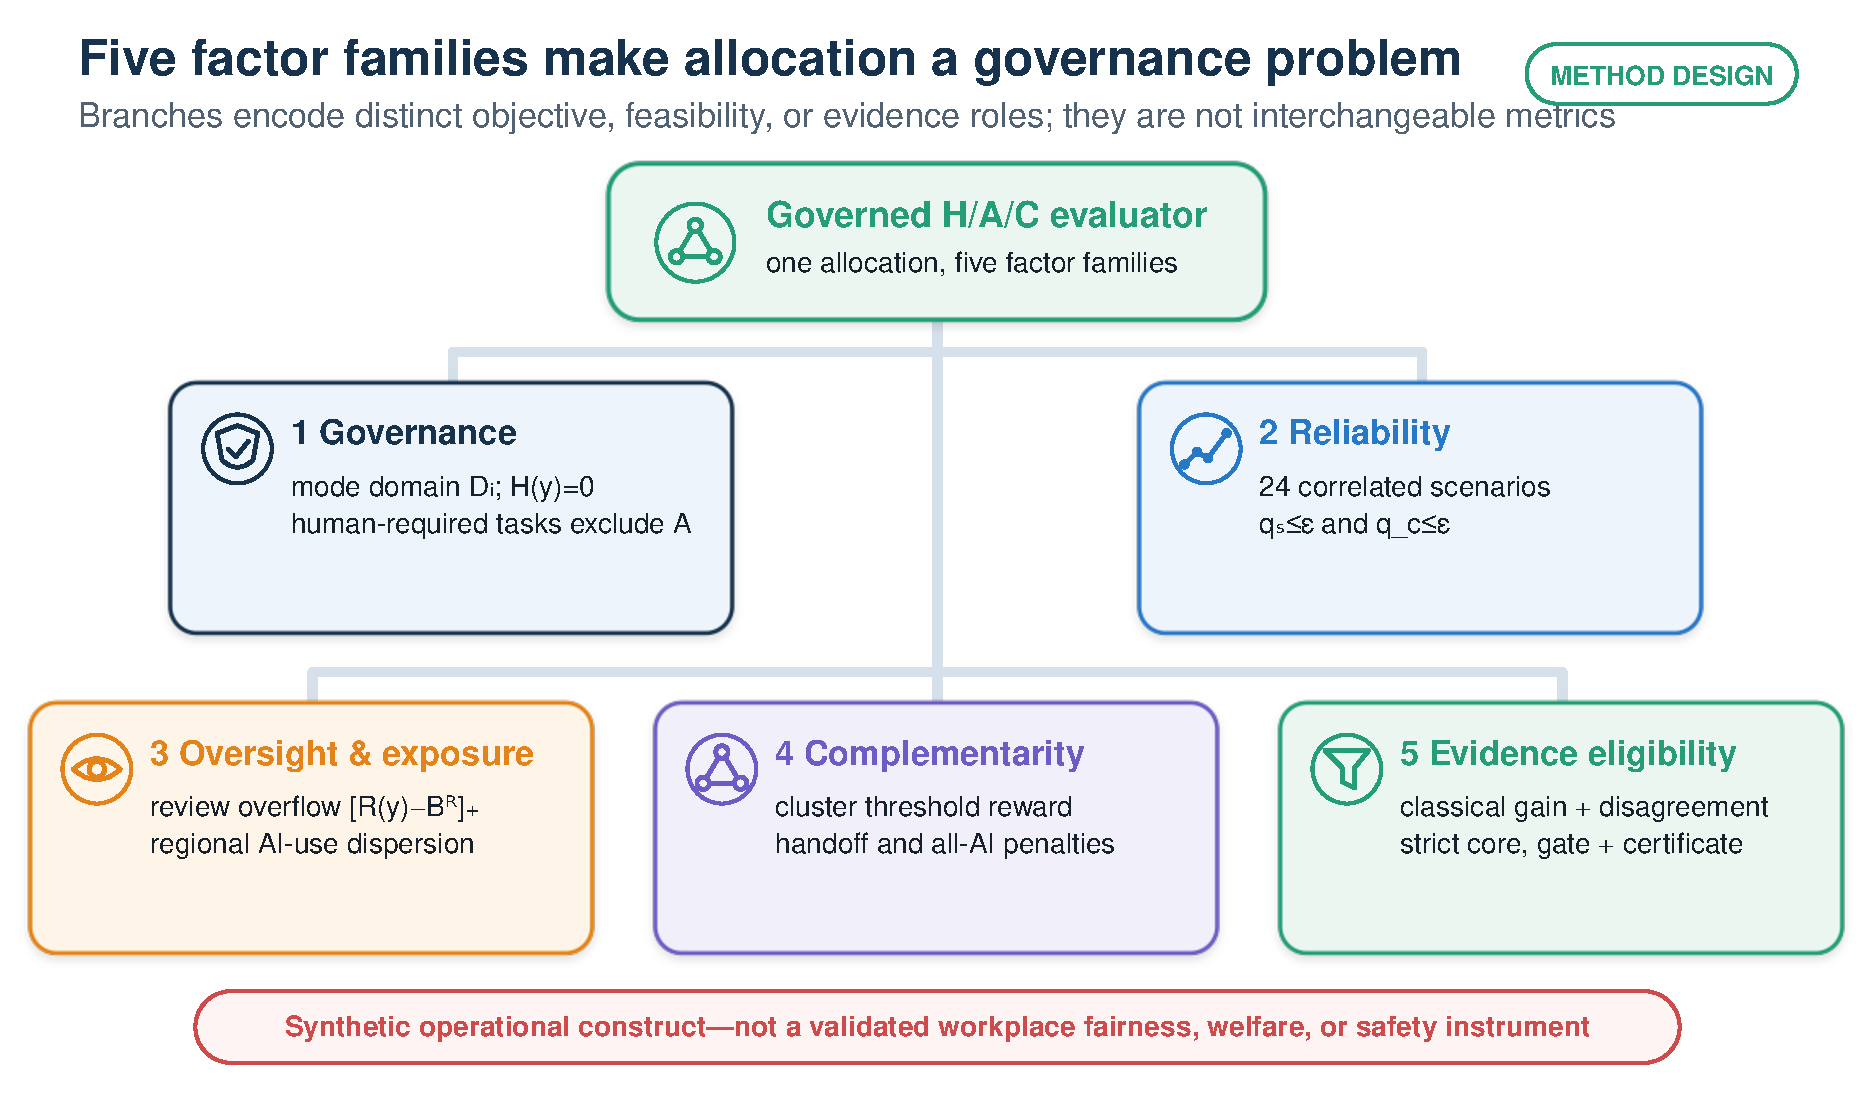
\includegraphics[width=\linewidth]{figs/fig2_benchmark_taxonomy.pdf}
  \caption{Five benchmark factor families. The exposure term is a coded dispersion regularizer, not a validated fairness construct; all variables and coefficients are specified in Appendix~\ref{app:benchmark}.}
  \label{fig:taxonomy}
\end{figure}


The five families in \cref{tab:factorfamilies,fig:taxonomy} are deliberately heterogeneous: governance, stochastic reliability, oversight/exposure, organizational complementarity, and evidence eligibility. Appendix~\ref{app:benchmark} gives every implemented formula, its plain-language meaning, status and literature connection. All numerical coefficients are frozen synthetic benchmark choices; none is presented as a learned social welfare weight or calibrated workplace threshold.

\section{The \UWCQ{} evidence-audit stack}
\label{sec:framework}

\paragraph{C: strong classical control and retained core.}
A per-task value-minus-cost seed is improved by best legal one-coordinate moves until convergence. Cluster destroy/repair then exactly enumerates one three-task cluster (occasionally plus one external task) for 18 iterations and two restarts. This is motivated by adaptive large-neighborhood search~\citep{ropke2006alns}, but we call the implemented method \emph{cluster repair} to avoid implying a broad ALNS benchmark. Let $y^G,y^C$ be the greedy and cluster incumbents, $\Delta=S(y^C)-S(y^G)$, $d=|I|^{-1}\sum_i\ind[y_i^G\ne y_i^C]$, and $v_R$ restart-score variance. Classical ambiguity is
\begin{equation}
 a=\min\!\left\{1,,2.8d+5\left[\frac{\Delta}{\max(|S(y^C)|,1)}\right]_+ +4\frac{\sqrt{v_R}}{\max(|S(y^C)|,1)}\right\}.
 \label{eq:ambiguity}
\end{equation}
Clusters are ranked by their complementarity/penalty magnitudes plus disagreement; four task indices $I_4$ are retained. Every assignment in $\prod_{i\in I_4}D_i$ is evaluated exactly with $y^C$ fixed outside $I_4$. The strict set $\mathcal Z=\{z:F(z,y^C_{-I_4})=1\}$ has at most $3^4=81$ states. If empty, the lowest 20\% by an explicit violation score is retained and marked fallback, never relabeled feasible.

\paragraph{W, U and Q: matched distributions.}
The warm state $z_W$ is the retained state nearest the cluster incumbent, and the normalized initial amplitude is
\begin{equation}
 \langle z|\psi_0\rangle\propto\exp[-.35d_H(z,z_W)].
 \label{eq:warm}
\end{equation}
The retained graph connects states differing by one mode; isolated nodes connect to their nearest retained neighbor. With energy $E(z)=-S(z,y^C_{-I_4})$, standardized diagonal cost Hamiltonian $H_C$ and mixer $H_M=-A_{\mathcal Z}$, the simulated state is
\begin{equation}
 |\psi_p(\boldsymbol\gamma,\boldsymbol\beta)\rangle=\prod_{\ell=1}^{p}e^{-i\beta_\ell H_M}e^{-i\gamma_\ell H_C}|\psi_0\rangle.
 \label{eq:qaoa}
\end{equation}
The uniform comparator uses $P_U(z)=1/|\mathcal Z|$. QAOA uses exact noiseless statevector probabilities. Both are sampled with replacement for 128 matched-budget draws. Primary quantum evidence is optimum mass $p^\star=\sum_{z:E(z)=E_{\min}}P(z)$; first-hit draw $T$ is a sampling proxy with misses coded 129, not wall-clock runtime.

\begin{table}[t]
\centering
\caption{The \textsc{U--W--C--Q} layers and their evidentiary roles.}
\label{tab:uwcq}
\scriptsize
\begin{tabularx}{\linewidth}{@{}p{0.07\linewidth}p{0.20\linewidth}p{0.31\linewidth}X@{}}
\toprule
Layer & Implemented object & Formula / metric & Role \\
\midrule
U & Uniform retained-state sampler & $P_U(z)=1/|\mathcal Z|$; 128 draws & Uninformed feasible-set comparator. \\
W & ALNS-nearest warm state & $\psi_0(z)\propto e^{-0.35d_H(z,z_W)}$ & Biases initial amplitude toward the incumbent. \\
C & Greedy, cluster repair, exact core, verifier & $\Delta=S_C-S_G$, $d=n^{-1}\sum_i\mathbf1[y_i^G\ne y_i^C]$ & Builds incumbent/core and checks accepted assignments. \\
Q & Retained-graph statevector QAOA & $\prod_{\ell=1}^p e^{-i\beta_\ell H_M}e^{-i\gamma_\ell H_C}|\psi_0\rangle$ & Tests probability concentration, not runtime advantage. \\
\bottomrule
\end{tabularx}
\end{table}

\begin{figure}[t]
  \centering
  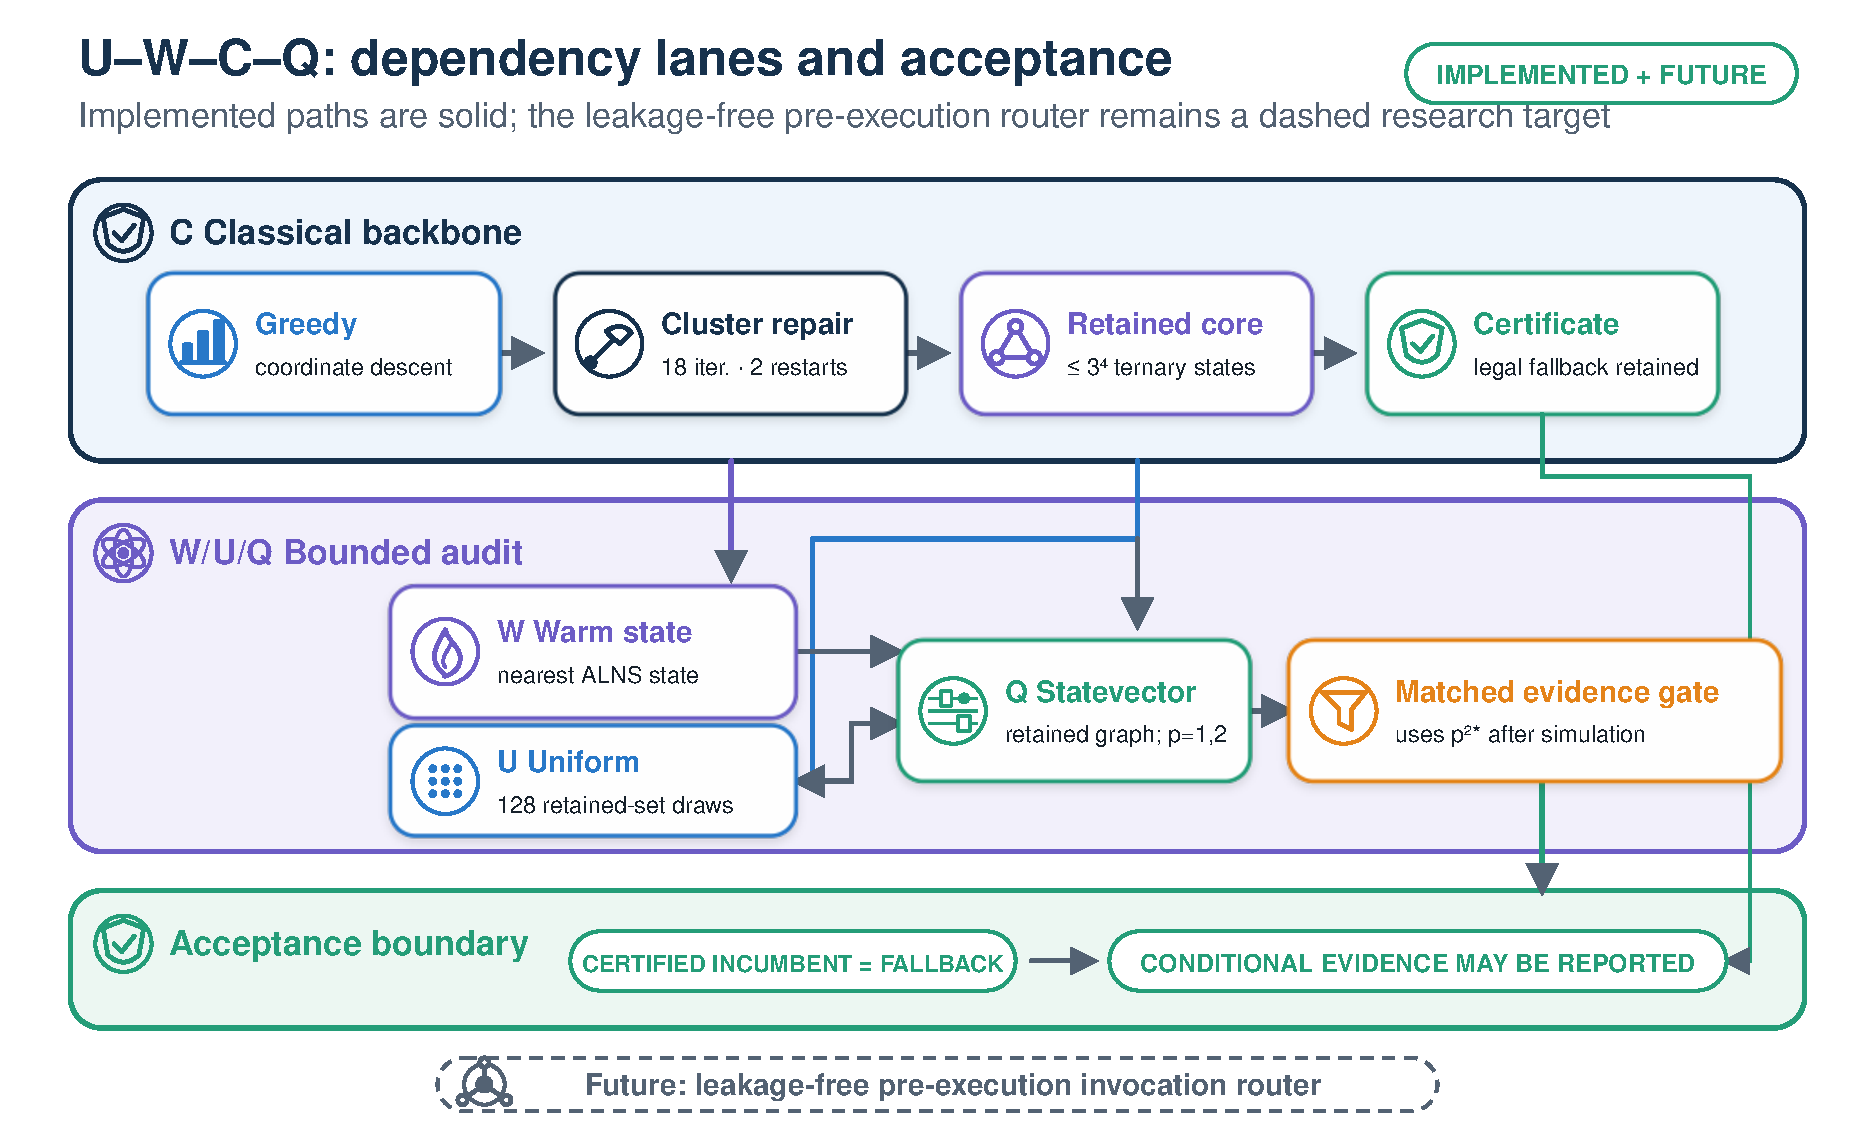
\includegraphics[width=\linewidth]{figs/fig3_uwcq_pipeline.pdf}
  \caption{Dependency lanes of \textsc{U--W--C--Q}. The classical backbone supplies the incumbent, retained core, and legal fallback; \textsc{W} and the retained set feed the bounded \textsc{U}/\textsc{Q} audit; the acceptance lane preserves classical certification. Because the evidence gate uses the simulated $p=2$ optimum mass, it is post-simulation and is not a cost-saving router. The dashed router is future work.}
  \label{fig:uwcq}
\end{figure}


\paragraph{Evidence gate and certificate.}
The frozen gate is
\begin{equation}
 g=F_{I_4}\land(a\ge.08)\land\left(p_2^\star\ge\max\{.18,1.4p_U^\star\}\right)\land(\Delta>10^{-6}\lor d\ge.05).
 \label{eq:gate}
\end{equation}
Crucially, $g$ consumes $p_2^\star$; it is a \emph{post-simulation evidence-eligibility indicator}, not a pre-execution invocation router. It therefore cannot reduce quantum cost. The final operational object in the present experiment remains the classically evaluated cluster-repair incumbent; the quantum branch audits the retained distribution and does not implement production candidate selection. Appendix~\ref{app:uwcq} provides the full formula glossary.

\section{Frozen experiment and inference}
\label{sec:experiments}

The preregistered factorial matrix crosses task counts $\{12,18\}$, four synthetic stress levels and four held-out seeds $\{101,211,307,401\}$, giving 32 instances; development seeds 11 and 23 are excluded. Each instance has 24 correlated scenarios, three regions, three-task clusters, service target .70, tolerance .20, and capacity scale .92. The retained core has four tasks. QAOA depths $p=1,2$ are frozen: $p=1$ receives a $13\times11=143$ point grid, whereas $p=2$ receives 30 seeded random trials. Their results are therefore descriptive, not an equal-optimizer-budget depth ablation.

For sampling, uniform and $p=2$ probabilities each receive 128 draws with frozen, method-specific seeds. Outcomes include classical gain/disagreement, strict-core availability, optimum mass, first-hit draws, near-optimal coverage, collaboration rate, evidence-gate status, explicit hard violations and composite feasibility. All 32 cases and nulls are retained. We report percentile 95\% bootstrap intervals over instances; contrasts use paired resampling with 10,000 draws. Appendix~\ref{app:protocol} gives the configuration digest, pseudocode, compute environment and exact reproduction commands.

\begin{table}[t]
\centering
\caption{Frozen 32-instance outcomes. Bracketed intervals are 95\% instance-level bootstrap intervals; paired effects use paired resampling.}
\label{tab:locked}
\scriptsize
\begin{tabularx}{\linewidth}{@{}p{0.31\linewidth}p{0.26\linewidth}X@{}}
\toprule
Metric & Result & Supported reading \\
\midrule
Strict feasible retained set & 30/32 = .938 [.844, 1.000] & Two cases used violation-ranked fallback. \\
Cluster repair beats greedy & 25/32 = .781 [.625, .906] & Mean gain 17.019; not an exhaustive classical comparison. \\
Post-simulation evidence gate & 9/32 = .281 [.125, .438] & Evidence is selective after simulation, not pre-routed. \\
Optimum probability, U $\rightarrow$ Q$_2$ & .0223 $\rightarrow$ .1522 & Paired difference .1299 [.0991, .1640]; ratio 6.831. \\
First-hit draws, U $\rightarrow$ Q$_2$ & 36.50 $\rightarrow$ 12.94 & Paired difference $-23.56$ [$-39.28,-8.69$]; misses coded 129. \\
Near-optimal coverage difference & +.0443 [$-.0208,.1120$] & Interval crosses zero; no clear coverage claim. \\
Explicit / composite feasibility & 0 mode violations; 27/32 feasible & Zero mode violations is narrower than zero composite failures. \\
Depth counterevidence & mean $p_1^\star=.2492$; $p_1>p_2$ on 28/32 & Search budgets differ; no monotone-depth conclusion. \\
\bottomrule
\end{tabularx}
\end{table}


The public snapshot was independently rerun without modifying it. Targeted benchmark tests pass (6/6), the frozen runner regenerates 32 rows, and all 704 values in the 22 fields shared by the current runner and the richer archived table match exactly (maximum absolute error 0). Eight archived diagnostic fields are no longer emitted by the current runner; we therefore claim exact \emph{shared-field} reproduction, not byte-identical CSV reproduction. This distinction is preserved in the supplementary audit manifest.

\section{Results: concentration with retained counterevidence}
\label{sec:results}

\paragraph{Classical structure and feasibility.}
Strict feasible retained states exist on 30/32 instances. Cluster repair improves over coordinate greedy on 25/32, with mean gain 17.019 (paired bootstrap CI [12.524,21.552]); collaboration rises descriptively from .475 to .664. These results justify a nontrivial classical control and show that workflow moves matter in the synthetic score. They do not establish superiority over mixed-integer programming, exhaustive full-instance optimization, or a broad ALNS portfolio. Moreover, only 27/32 cluster incumbents satisfy the composite feasibility predicate: five exceed review, service-scenario, or capacity-scenario tolerance, although all 32 have zero explicit disallowed-mode violations.

\paragraph{Conditional statevector signal.}
Mean exact optimum mass is .0223 under uniform retained-state sampling and .1522 under $p=2$ QAOA, a ratio of 6.831. The paired difference is .1299 with 95\% CI [.0991,.1640], and $p=2$ exceeds uniform on 30/32 instances. Under the frozen 128-draw simulations, mean first hit changes from 36.50 to 12.94; the paired difference is $-23.56$ draws [${-39.28},{-8.69}$]. Because a miss is coded as 129 and each method uses a single frozen draw sequence per instance, this is a matched sample-efficiency proxy rather than latency. The near-optimal coverage difference is +.0443 [${-.0208},.1120$], so its interval crosses zero and supports no clear coverage claim.

\begin{figure}[t]
  \centering
  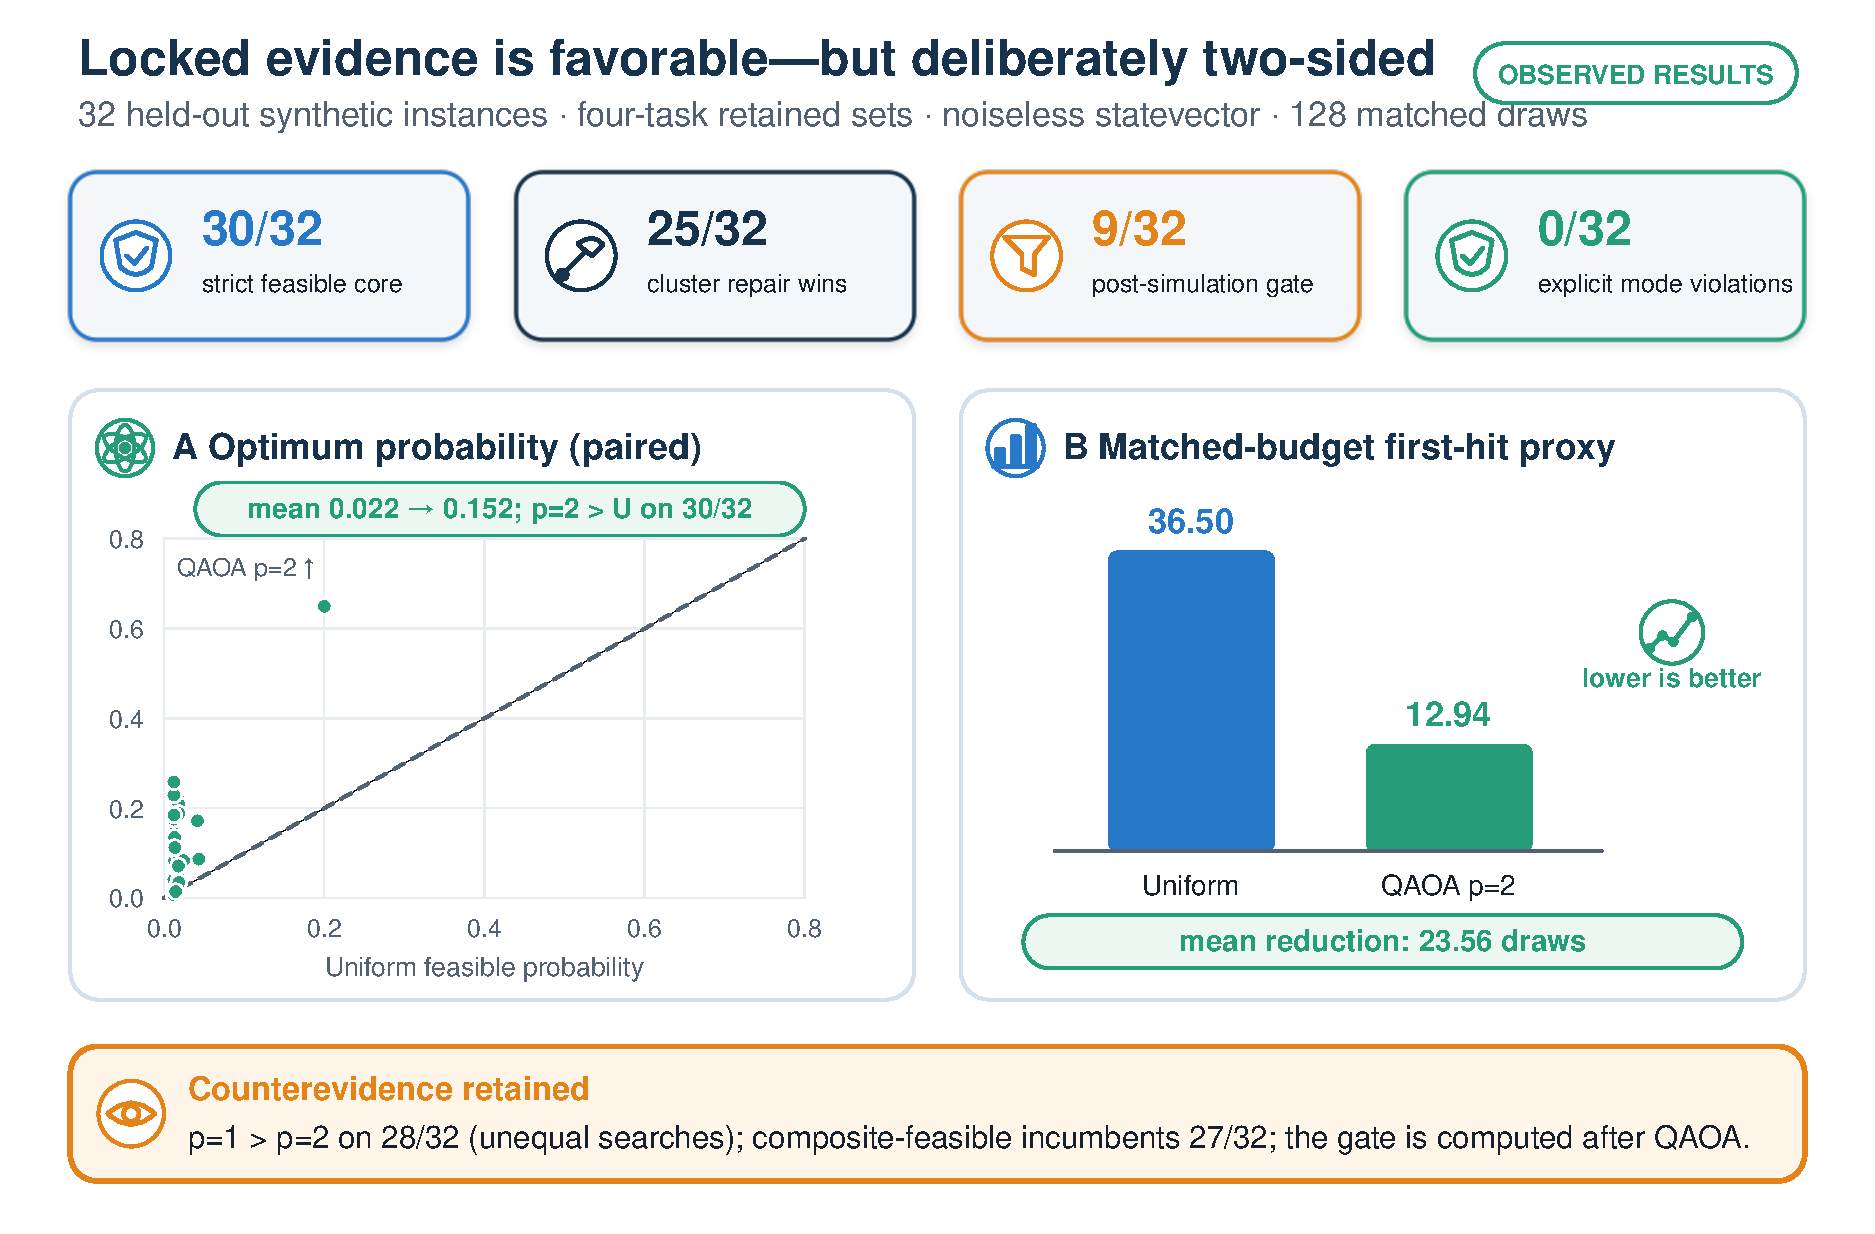
\includegraphics[width=\linewidth]{figs/fig5_results_dashboard.pdf}
  \caption{Frozen results. Panel A plots paired instance-level optimum masses; Panel B shows the matched-draw first-hit proxy. The orange strip preserves counterevidence needed to interpret depth, feasibility, and the post-simulation gate honestly.}
  \label{fig:results}
\end{figure}


\paragraph{Why ``selective'' remains an agenda, not a deployed policy.}
Only 9/32 cases satisfy the post-simulation gate. Ordered failures are 2 with no strict core, 7 with low classical ambiguity, and 14 with insufficient $p=2$ concentration. This partition is scientifically useful because it rejects a universal-use narrative. However, the gate observes the very quantum statistic whose computation a deployment router would decide whether to purchase. Calling it pre-execution ``adoption'' would therefore be target leakage. A credible invocation policy must learn or specify a decision from pre-simulation features and be frozen on separate instances.

\paragraph{Depth is counterevidence, not a success story.}
Mean $p=1$ optimum mass is .2492, and $p=1>p=2$ on 28/32 cases. Since $p=1$ receives 143 grid points while $p=2$ receives only 30 random candidates, neither circuit depth nor the parameter optimizer is isolated. The honest conclusion is that the frozen $p=2$ distribution concentrates probability relative to uniform, while deeper-is-better is unsupported. This pattern is consistent with the broader caution that variational performance depends on landscape, initialization and optimization budget~\citep{zhou2020qaoa,cerezo2021variational,blekos2024review}.

\begin{table}[t]
\centering
\caption{Reviewer-facing claim boundary.}
\label{tab:claims}
\scriptsize
\begin{tabularx}{\linewidth}{@{}p{0.21\linewidth}XX@{}}
\toprule
Risk & Defensible statement & Evidence still required \\
\midrule
``Quantum advantage'' & Conditional noiseless statevector concentration on frozen four-task retained sets. & QPU execution; wall-clock, energy and scaling comparisons. \\
``Selective invocation'' & A post-simulation evidence-eligibility gate partitions the frozen results. & A leakage-free pre-execution router evaluated out of sample. \\
``Zero violations'' & All incumbents have zero explicit disallowed-mode violations. & Composite feasibility holds for 27/32; deployment needs safety validation. \\
``Fair allocation'' & A regional AI-exposure dispersion regularizer is implemented. & Stakeholder-defined fairness constructs and disaggregated field outcomes. \\
``Depth helps'' & Both $p=1$ and $p=2$ were frozen and reported. & Equal-budget optimization, noise-aware sweeps and larger cores. \\
``First'' & Scoped review found no prior reproducible integration of all listed controls. & A systematic review could support a stronger priority claim. \\
\bottomrule
\end{tabularx}
\end{table}


\paragraph{Integrated significance.}
The benchmark contributes more than a QAOA toy by forcing the quantum comparison to inherit governance and stochastic feasibility from a shared evaluator. Conversely, the statevector result contributes less than a deployment demonstration: there is no QPU noise, transpilation, wall-clock or energy accounting, and the four-task retained space is exactly enumerable. The defensible result is a reproducible \emph{candidate concentration signal conditional on classical decomposition and certification}. Its value is methodological: it shows which controls, nulls and distinctions a future advantage claim must survive.

\section{Open interdisciplinary questions}
\label{sec:agenda}

\begin{figure}[t]
  \centering
  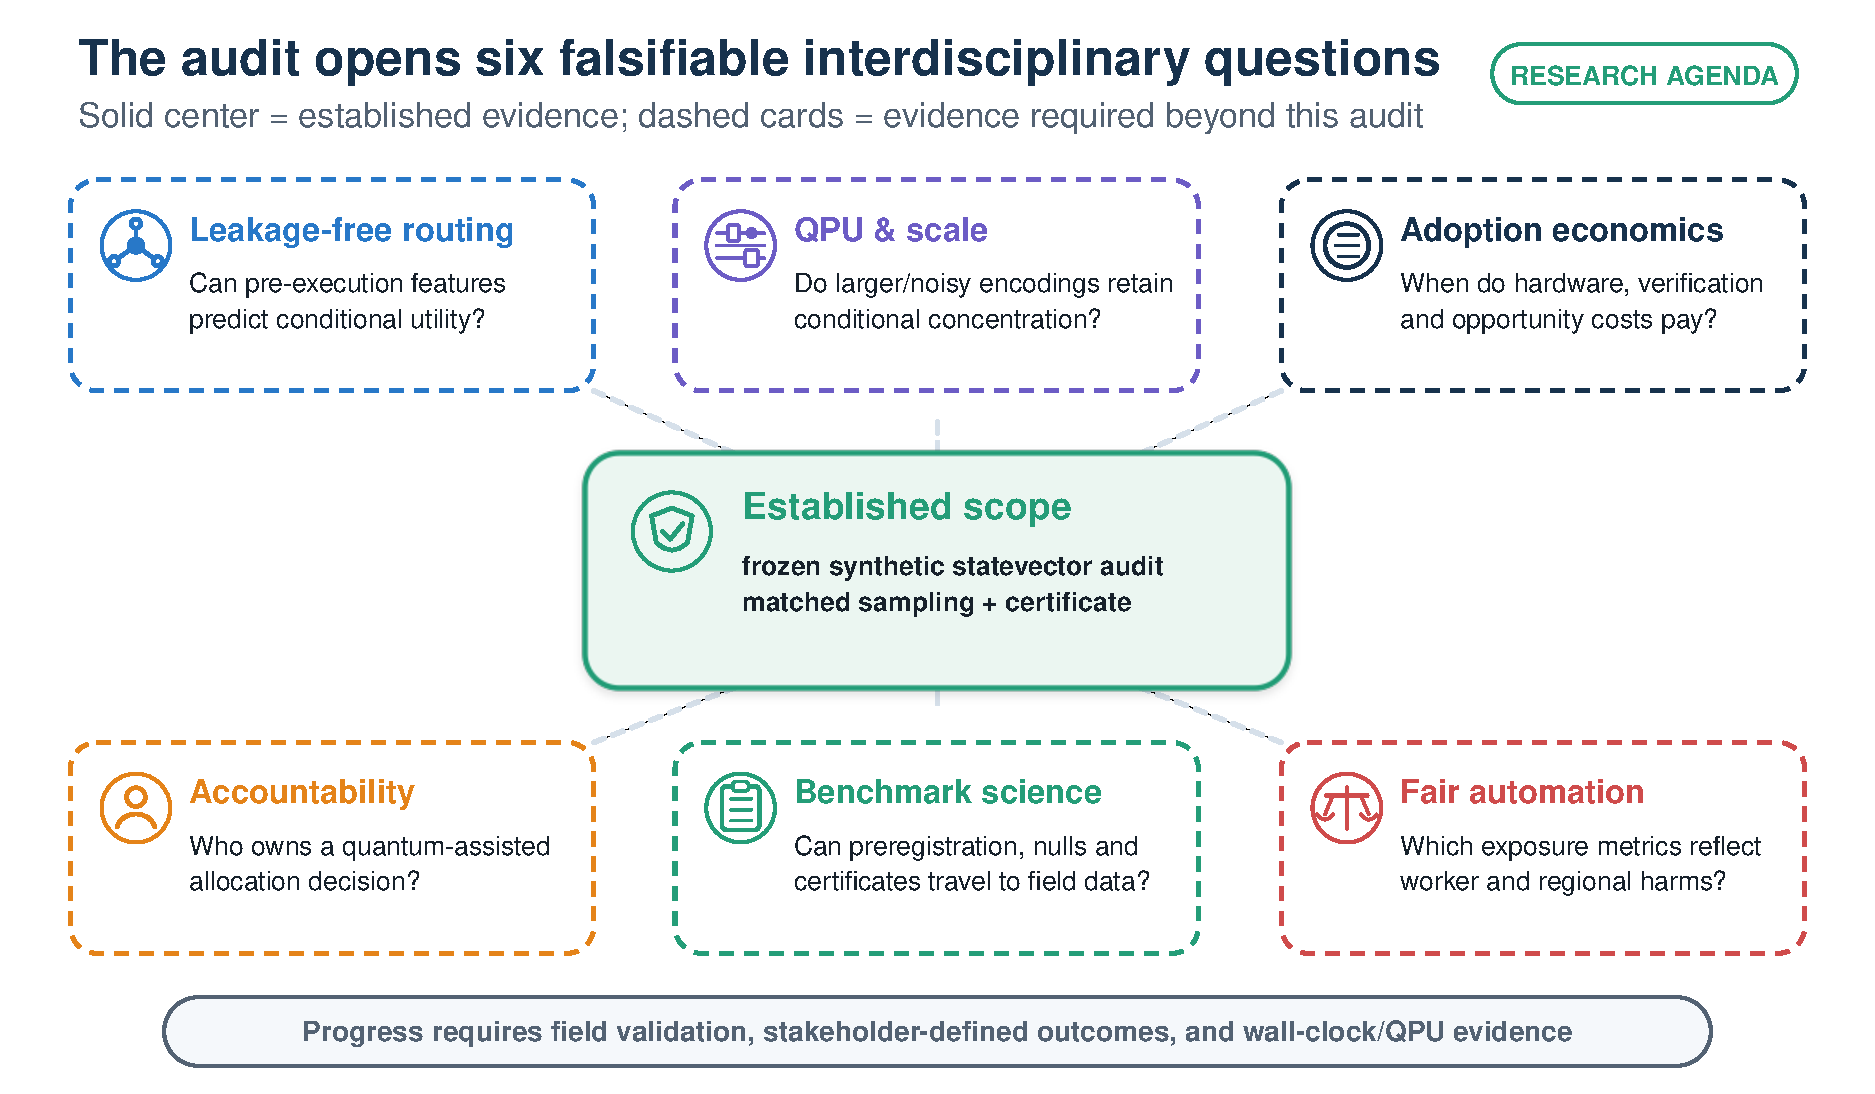
\includegraphics[width=\linewidth]{figs/fig6_open_questions_map.pdf}
  \caption{Research agenda induced by the evidence boundary. The solid center is established here; dashed cards require new field, governance, economic, or quantum-hardware evidence.}
  \label{fig:agenda}
\end{figure}


The evidence boundary exposes six research programs. \textbf{(1) Leakage-free routing:} can pre-execution instance features predict incremental quantum utility under locked, out-of-sample evaluation, connecting selective prediction and algorithm selection~\citep{geifman2017selective,rice1976algorithm,kotthoff2014algorithm}? \textbf{(2) Adoption economics:} when do QPU access, engineering, verification, delay and opportunity costs justify invocation? This is a bounded-rationality and organizational-contracting problem, not merely an algorithmic ratio~\citep{simon1955behavioral,hart1990property}. \textbf{(3) Accountability:} who owns a classically certified but quantum-influenced allocation, and what evidence should a governance system retain~\citep{nist2023airmf,iso42001}? \textbf{(4) Fair automation:} which stakeholder-defined exposure, workload and labor outcomes should replace our simple dispersion term~\citep{selbst2019fairness,bai2022algorithmic}? \textbf{(5) QPU and scale:} does conditional concentration survive larger encodings, noise, compilation and equal-budget optimizer sweeps~\citep{preskill2018nisq,bharti2022nisq}? \textbf{(6) Benchmark science:} can preregistration, null retention and certificates extend to privacy-preserving field data while maintaining reproducibility~\citep{pineau2021reproducibility}? These are falsifiable next steps; none is answered by the present synthetic statevector experiment.

\section{Limitations, ethics, and conclusion}
\label{sec:limitations}

The evaluator is synthetic: costs, success rates, disruption processes and penalty weights are not estimated from workers, customers or organizations. No human subjects or personal data are used. Regional AI exposure dispersion is not a fairness guarantee, collaboration rate is not a welfare outcome, and zero disallowed-mode violations is not workplace safety. A poorly chosen real deployment could still automate unequally, overload reviewers, obscure responsibility or displace work. Any field study therefore requires stakeholder participation, privacy governance, domain-specific outcome validity, and human override; NIST and ISO references are framing resources, not certifications~\citep{nist2023airmf,iso42001,iso23894}.

Quantum limitations are equally sharp: four retained ternary variables, exact enumeration, noiseless statevectors, no gate decomposition, no QPU, no noise, no timing and unequal depth-search budgets. Uniform sampling is a controlled distributional baseline, not the strongest possible classical sampler. The cluster-repair method is stronger than a trivial baseline but not a comprehensive solver portfolio. Bootstrap intervals quantify variation across the 32 frozen instances, not generalization to a population of organizations.

Within those limits, Q-OPS demonstrates a disciplined pattern for quantum-assisted organizational research: formulate governance before invocation, make classical controls strong and inspectable, compare distributions on the same retained set and budget, retain adverse results, and keep a classical acceptance boundary. The frozen evidence supports conditional statevector concentration and a lower first-hit draw proxy at $p=2$ relative to uniform, while rejecting claims about monotone depth, universal invocation and complete feasibility. That two-sided result is the paper's central contribution and a reproducible foundation for the open agenda in \cref{sec:agenda}.


\bibliographystyle{plainnat}
\bibliography{references}

\appendix
\section{Benchmark formulas, meanings, and precedents}
\label{app:benchmark}

This appendix distinguishes four evidence statuses: \emph{implemented} means the public evaluator computes the quantity; \emph{synthetic} means its coefficient is generated or frozen rather than estimated from field data; \emph{interpretive} means we supply a real-world analogy; and \emph{validated} is deliberately not asserted for organizational welfare, safety, or fairness.

For scenario $\omega$, let $D_\omega$ be demand, $h_{r\omega}$ and $a_{r\omega}$ regional human/AI factors, and $u_\omega$ the common AI shock. With clipped success to $[0,1]$,
\begin{align}
s_{i\omega}(\Hmode)&=\bar s_i^H h_{r(i)\omega}, & (\ell^H,\ell^A)(\Hmode)&=(1,0),\\
s_{i\omega}(\Amode)&=\bar s_i^A a_{r(i)\omega}u_\omega, &(\ell^H,\ell^A)(\Amode)&=(0,1),\\
s_{i\omega}(\Cmode)&=\bar s_i^C(.55h_{r(i)\omega}+.45a_{r(i)\omega})(.985+.015u_\omega),
 &(\ell^H,\ell^A)(\Cmode)&=(.45,.65).
\end{align}
Regional overflow is the sum of positive excesses over scenario-scaled human and AI capacities:
\begin{equation}
 O_\omega(y)=\sum_r\left[L^H_{r\omega}(y)-B^H_rh_{r\omega}\right]_+ +
 \left[L^A_{r\omega}(y)-B^A_ra_{r\omega}\right]_+,
\end{equation}
where $L^x_{r\omega}=\sum_{i:r(i)=r}d_iD_\omega\ell^x(y_i)$. These equations correct a tempting but inaccurate simplification: the service constraint is aggregate and scenario-based, not a separate chance constraint for every task.

\begingroup
\small
\setlength{\tabcolsep}{3pt}
\begin{longtable}{@{}p{0.13\linewidth}p{0.25\linewidth}p{0.25\linewidth}p{0.28\linewidth}@{}}
\caption{Complete benchmark formula glossary. Every row is implemented in the frozen evaluator.}\label{tab:benchmarkglossary}\\
\toprule
Factor & Implemented definition & Plain-language / real-world role & Evidence and literature \\
\midrule
\endfirsthead
\toprule
Factor & Implemented definition & Plain-language / real-world role & Evidence and literature \\
\midrule
\endhead
Mode & $y_i\in\{H,A,C\}$; $A\notin D_i$ for human-mandatory $i$ & Each task is human-only, AI-only, or collaborative; some retain human responsibility. & Directly enumerated domain; human--AI interaction design motivates explicit authority boundaries~\citep{amershi2019humanai,seeber2020machines}. \\
Hard violations & $H(y)=\sum_i\mathbf1[y_i\notin D_i]$ & Counts disallowed assignments; this is narrower than composite feasibility. & Shared final check; governance context~\citep{nist2023airmf,iso42001}. \\
Base cost & $C(y)=\sum_i d_i c_{i,y_i}$ & Duration-weighted cost of the chosen operating mode. & Scenario-independent term in the evaluator; resource allocation tradition~\citep{gans2003callcenters}. \\
Review load & $R(y)=\sum_i r_i(\mathbf1[y_i=A]+.25\mathbf1[y_i=C])$ & AI-only work consumes a full review unit; collaboration consumes one quarter. & Synthetic coefficient, not empirically calibrated; makes oversight capacity explicit~\citep{nist2023airmf}. \\
Review overflow & $R_+(y)=[R(y)-B_R]_+$ & Review demand above the available audit budget. & Penalized by 9 in the score; operational bottleneck construct. \\
Cluster reward & $\sum_k B_k\mathbf1[n_k^C\ge h_k]$ & Collaboration creates value only after a workflow-level threshold. & Implemented clusters of at most three tasks; complementarity motivation~\citep{seeber2020machines,fuegener2026complementarity}. \\
All-AI penalty & $\sum_k A_k\mathbf1[\forall i\in k:y_i=A]$ & A fully automated workflow incurs a governance/robustness cost. & Synthetic penalty, increasing with stress level; not a causal harm estimate. \\
Handoff penalty & $\sum_k J_k(|\{y_i:i\in k\}|-1)_+$ & More modes inside one cluster create coordination overhead. & Implemented synthetic workflow-mixing cost; the coefficient is not empirically calibrated. \\
AI exposure dispersion & $P_{\rm exp}(y)=2\operatorname{sd}_{r}(a_r)$, $a_r=|I_r|^{-1}\sum_{i\in I_r}\mathbf1[y_i=A]$ & Penalizes uneven AI-only rates across modeled regions. & Coded diagnostic, \emph{not} validated fairness; sociotechnical cautions~\citep{selbst2019fairness,mehrabi2021fairness,bai2022algorithmic}. \\
Scenario loads & $L^H_{r\omega}=\sum_{i\in r}d_iD_\omega\ell^H(y_i)$, $L^A_{r\omega}=\sum_{i\in r}d_iD_\omega\ell^A(y_i)$, with $(\ell^H,\ell^A)=(1,0),(0,1),(.45,.65)$ & Human and AI capacity draw changes by mode and correlated demand scenario. & Exact frozen coefficients; chance-constrained operations motivation~\citep{charnes1959chance,gans2003callcenters}. \\
Scenario success & $s_{i\omega}=\bar s_{i,y_i}$ times regional human/AI factors and AI shock; collaboration blends factors $.55/.45$ & Mode success changes with regional and common disruptions. & Exact generator/evaluator equations in Appendix~\ref{app:benchmark}; synthetic, not field-estimated. \\
Service risk & $q_s(y)=|\Omega|^{-1}\sum_\omega\mathbf1[\rho_\omega(y)<.70]$, with $\rho_\omega=\sum_i p_i s_{i\omega}/\sum_i p_i$ & Fraction of scenarios whose priority-weighted service falls below target. & Target .70, tolerance $\epsilon=.20$; empirical chance constraint~\citep{charnes1959chance}. \\
Capacity risk & $q_c(y)=|\Omega|^{-1}\sum_\omega\mathbf1[O_\omega(y)>0]$ & Fraction of scenarios with any regional human/AI capacity overflow. & Tolerance $\epsilon=.20$; overflow also priced inside scenario value. \\
Scenario value & $V_\omega(y)=\sum_i v_i s_{i\omega}-C(y)-4O_\omega(y)$ & Expected delivered value net of cost and scenario overflow. & Averaged over 24 scenarios. \\
Composite score & $S(y)=\bar V+\text{cluster reward}-\text{cluster penalties}-P_{\rm exp}-9R_+-600H-150[q_s-.2]_+-45[q_c-.2]_+$ & A single score ranks assignments while retaining explicit diagnostics. & Exact frozen implementation; coefficients are benchmark parameters, not learned welfare weights. \\
Composite feasible & $F(y)=\mathbf1[H=0,R_+=0,q_s\le.2,q_c\le.2]$ & Requires mode legality, review capacity, service reliability and capacity reliability. & Used for strict retained states and reported separately from hard-mode legality. \\
Collaboration rate & $n^{-1}\sum_i\mathbf1[y_i=C]$ & Describes how often the collaborative mode is selected. & Descriptive outcome only; it is not itself a success metric. \\
\bottomrule
\end{longtable}
\endgroup


\paragraph{Generator distributions.}
The generator assigns three-task clusters, up to three modeled regions, task values in $[9,18]$, human success in $[.94,.99]$, AI success based on $[.84,.955]$ with a sensitivity decrement, and collaborative success above the better base mode by a sampled margin, capped at .997. Costs, capacities, review requirements, cluster coefficients and disruption strength are seeded. The four stress levels increase sensitive-task prevalence, outage probability and selected penalties. These ranges define a controlled stress test, not an empirical model of any named industry.

\section{Complete \UWCQ{} formula glossary}
\label{app:uwcq}

The mnemonic is not execution order. The classical layer encloses the experiment: it produces the incumbent and retained set, while the same evaluator verifies the final assignment. The warm layer feeds Q, and U/Q form a paired distributional comparison. \Cref{fig:uwcq} visualizes this dependency; \cref{tab:uwcqglossary} records every implemented strategy and metric.

\begingroup
\small
\setlength{\tabcolsep}{3pt}
\begin{longtable}{@{}p{0.14\linewidth}p{0.25\linewidth}p{0.25\linewidth}p{0.27\linewidth}@{}}
\caption{Complete \textsc{U--W--C--Q} strategy and metric glossary.}\label{tab:uwcqglossary}\\
\toprule
Object & Formula / implementation & Intuitive definition & Use and precedent \\
\midrule
\endfirsthead
\toprule
Object & Formula / implementation & Intuitive definition & Use and precedent \\
\midrule
\endhead
Individual seed & $\arg\max_{m\in D_i}(v_i\bar s_{im}-d_ic_{im})$ per task & Myopic value-minus-cost initialization. & Starting point for coordinate descent. \\
Greedy control & Repeated best legal one-task move until no $S$ improvement & Stronger than an all-human or random straw baseline. & Classical control; local-search precedent. \\
Cluster repair & Exact enumeration of one three-task cluster, sometimes plus one external task, for 18 iterations and 2 restarts & Destroy/repair coordinated assignments inside a small neighborhood. & Inspired by ALNS~\citep{ropke2006alns}; the implementation is intentionally reported as \emph{cluster repair}, not a comprehensive ALNS suite. \\
Classical gain & $\Delta=S(y^C)-S(y^G)$ & Improvement of cluster repair over greedy. & One ambiguity signal; mean and win rate are frozen outcomes. \\
Disagreement & $d=n^{-1}\sum_i\mathbf1[y_i^G\ne y_i^C]$ & How differently the two classical procedures allocate tasks. & A second ambiguity signal. \\
Ambiguity & $a=\min\{1,2.8d+5[\Delta/\max(|S_C|,1)]_++4\sqrt{v_R}/\max(|S_C|,1)\}$ & Normalized evidence that the classical landscape is contested. & Threshold $.08$; diagnostic, not calibrated probability. Algorithm selection context~\citep{rice1976algorithm,kotthoff2014algorithm}. \\
Core score & $B_k+A_k+J_k\max(1,|k|-1)+5\bar d_k$ & Ranks clusters by complementarity, penalties and disagreement. & Selects four task indices; not a learned selector. \\
Retained set & Enumerate $\prod_{i\in I}D_i$; keep $F(y)=1$ & Exact small-core assignments that remain feasible with the incumbent outside the core. & At most $3^4=81$ states. \\
Fallback set & If no strict state, retain lowest 20\% of $20H+2R_++q_s+q_c$ & Keeps a least-violating diagnostic set when strict feasibility fails. & Used on 2/32 instances; never relabeled feasible. \\
Retained graph & $A_{zz'}=1$ for one-mode Hamming neighbors; connect isolated nodes to nearest retained state & Mixer moves only among retained states. & Feasible alternating-operator motivation~\citep{hadfield2019alternating,sawaya2023mixers}. \\
Warm state & $z_W=\arg\min_{z\in\mathcal Z}d_H(z,y^C_I)$; $\psi_0(z)\propto e^{-.35d_H(z,z_W)}$ & Starts near the cluster-repair incumbent while retaining support elsewhere. & Warm-start motivation~\citep{egger2021warm}. \\
Hamiltonians & $H_C=\operatorname{diag}((E-\bar E)/\sigma_E)$, $E=-S$; $H_M=-A$ & Phase by standardized cost; mix along retained edges. & Statevector implementation; no gate compilation or noise model. \\
QAOA state & $|\psi_p\rangle=\prod_{\ell=1}^p U_M(\beta_\ell)U_C(\gamma_\ell)|\psi_0\rangle$ & Alternates mixer and cost evolution, with $U_X(t)=e^{-itH_X}$. & QAOA/alternating-operator line~\citep{farhi2014qaoa,hadfield2019alternating,blekos2024review}. \\
Parameter search & $p=1$: $13\times11$ grid; $p=2$: 30 seeded random trials; lexicographic objective $(\mathbb E[E],-M_{.05},-p^\star)$ & Frozen but unequal searches at the two depths. & Supports reporting each depth, not a causal depth comparison. \\
Uniform baseline & $P_U(z)=1/|\mathcal Z|$ & Uninformed sampling on the same retained set. & Isolates concentration from feasibility filtering. \\
Optimum mass & $p^\star=\sum_{z:E(z)=E_{\min}}P(z)$ & Probability of drawing any exactly optimal retained state. & Primary statevector concentration metric. \\
Near-optimal mass & $M_{.05}=\sum_{z\in\mathcal N_{.05}}P(z)$, $\mathcal N_{.05}=\{E\le E_{\min}+.05\,\mathrm{range}(E)\}$ & Probability inside a 5\%-of-range energy band. & Secondary optimizer tie-break and descriptive metric. \\
First hit & $T=\min\{b:z_b\text{ optimal}\}$; $T=129$ on a miss, budget 128 & Draw index of the first optimum under one seeded matched sample. & Sample-efficiency proxy, not wall-clock runtime. \\
Coverage & distinct sampled near-optimal states / all near-optimal retained states & Diversity inside the near-optimal band. & Paired difference interval crosses zero. \\
Evidence gate & $F_I\land a\ge.08\land p_2^\star\ge\max(.18,1.4p_U^\star)\land(\Delta>0\lor d\ge.05)$ & Flags frozen instances with strict feasibility, ambiguity and sufficient simulated concentration. & Computed \emph{after} QAOA; not an invocation policy. \\
Verification & Re-evaluate the accepted full assignment with the shared scenario evaluator & Separates quantum evidence from operational acceptance without implying a third-party certificate. & In the current experiment the cluster-repair incumbent remains the final/fallback assignment. \\
\bottomrule
\end{longtable}
\endgroup


\paragraph{Parameter-selection objective.}
For every frozen parameter candidate, statevector probabilities are ranked lexicographically by expected energy, then negative near-optimal mass, then negative exact-optimum mass. Thus $p^\star$ is not the sole optimization objective. The $p=1$ grid and $p=2$ random search also have unequal cardinality. Reporting the strong $p=1$ result is therefore part of the audit rather than an ablation.

\paragraph{No production quantum assignment.}
The implementation computes an exact best retained-core state for reference and distributional sampling metrics, but it does not replace the cluster-repair incumbent with a sampled quantum candidate. ``Classical certificate'' in this paper means that any accepted full assignment is evaluated by the common scenario evaluator; in the frozen run, the operational incumbent remains classical. This distinction prevents probability concentration from being misreported as an implemented end-to-end policy improvement.

\section{Frozen protocol and pseudocode}
\label{app:protocol}

\begin{table}[h]
\centering
\caption{Frozen experimental protocol.}
\label{tab:protocol}
\small
\begin{tabularx}{\linewidth}{@{}p{0.28\linewidth}X@{}}
\toprule
Component & Frozen value \\
\midrule
Factorial matrix & $n\in\{12,18\}$; stress/doping $\in\{0,1,2,3\}$; seeds $\{101,211,307,401\}$; 32 instances total \\
Scenarios & 24 correlated scenarios per instance; service target .70; tolerance .20; capacity scale .92 \\
Classical & Coordinate greedy; cluster destroy/repair, 18 iterations, 2 restarts \\
Retained core & 4 variables; ternary legal domains; exact retained-core enumeration; at most 81 states \\
Quantum & Noiseless feasible-subspace statevector; $p=1,2$; $p=1$ grid 143 points; $p=2$ seeded random search 30 points \\
Sampling & 128 replacement draws per U/Q distribution; different frozen seeds; miss coded 129 \\
Inference & Instance is the paired unit; percentile paired bootstrap; 10,000 resamples; all prespecified nulls retained \\
Config digest & \texttt{7f07459abc9e686934be1ee022768eb82}\\[-1mm]
& \texttt{a9687137cc86d4d7ea0b7727715e53c} \\
Source snapshot & Anonymous frozen implementation artifact; identifying commit retained in the external audit only \\
\bottomrule
\end{tabularx}
\end{table}


\paragraph{Locked runner.}
For each tuple $(n,\text{stress},\text{seed})$ in the frozen matrix:
\begin{enumerate}[leftmargin=2em,itemsep=1pt,topsep=2pt]
\item generate the synthetic tasks, clusters, capacities and 24 correlated scenarios;
\item run coordinate greedy and cluster repair, preserving scores, assignments and restart variance;
\item rank clusters, select four task indices, exactly enumerate their legal assignments, and retain composite-feasible states (or explicitly marked least-violating fallback states);
\item compute the uniform distribution, the warm state, and optimized noiseless QAOA distributions at $p=1,2$;
\item draw 128 samples from uniform and $p=2$ with frozen method-specific seeds;
\item calculate ambiguity and the post-simulation evidence gate; and
\item serialize every instance, including null and gate-negative cases, before aggregate bootstrap inference.
\end{enumerate}

\paragraph{Inference.}
The instance is the paired unit. For a contrast $d_j$ over $j=1,\ldots,32$, the reported percentile interval is the 2.5th and 97.5th percentiles of $10{,}000$ means formed by resampling instance indices with replacement. Seeds 7001--7004 are fixed for gain, optimum-mass difference, first-hit difference and coverage difference. These intervals quantify the frozen matrix, not a random sample of real organizations.

\paragraph{Compute.}
The independent verification used Python 3.12.13 and NumPy 2.3.5 on Linux 6.18.35, an AMD EPYC 9V74 allocation with 9 logical CPUs and 21~GiB RAM. The complete 32-instance locked rerun took 31.980 seconds wall-clock and no GPU. Runtime is an environment/load observation, not an advantage metric. The archived manifest records Python 3.13.5 and NumPy 2.3.5 but not original CPU or wall time; this missing historical metadata is disclosed rather than reconstructed.

\section{Additional results and diagnostic partitions}
\label{app:additional}

\begin{table}[h]
\centering
\caption{Ordered post-simulation evidence-gate partition.}
\label{tab:gatepartition}
\small
\begin{tabularx}{\linewidth}{@{}p{0.34\linewidth}p{0.16\linewidth}X@{}}
\toprule
First failing/succeeding condition & Count & Interpretation \\
\midrule
No strict feasible retained state & 2 & Violation-ranked fallback; cannot support strict-core evidence. \\
Classical ambiguity below .08 & 7 & Strong classical methods give little reason to focus on disagreement. \\
Concentration below frozen threshold & 14 & QAOA $p=2$ does not meet both absolute and relative mass thresholds. \\
All evidence conditions pass & 9 & Post-simulation evidence-positive subset; still not a deployment decision. \\
\bottomrule
\end{tabularx}
\end{table}


\paragraph{Depth and matched draws.}
Across instances, mean optimum masses are .022278 (uniform), .249182 ($p=1$), and .152190 ($p=2$). The $p=2$ value exceeds uniform on 30/32; $p=1$ exceeds $p=2$ on 28/32. Since the parameter searches are unequal and selected by expected energy before optimum mass, this is a warning against interpreting depth as the sole causal factor.

Uniform and $p=2$ near-optimal coverage means are .919271 and .963542. Their paired mean difference .044271 has 95\% interval [$-.020833,.111979$]. We therefore report the direction but make no positive coverage claim. The first-hit means of 36.50 and 12.9375 are sensitive to the frozen draw stream and miss code; they complement, rather than replace, the exact probability-mass result.

\paragraph{Feasibility decomposition.}
Thirty instances have at least one strict feasible retained state; two use fallback states. All 32 cluster-repair incumbents have zero explicit disallowed-mode violations, while 27 satisfy the stricter conjunction of review capacity and empirical service/capacity tolerances. Any abstract phrase ``zero final hard violations'' should be read as zero mode-domain violations only.

\paragraph{Gate interpretation.}
The ordered partition in \cref{tab:gatepartition} prevents double counting. Its 9 positive instances meet all frozen predicates after QAOA. A real invocation router would have to replace $p_2^\star$ with pre-execution features and be evaluated on new held-out instances. Until then, ``gate rate'' is an evidence summary, not a rate of saved QPU calls.

\section{Reproducibility and claim traceability}
\label{app:reproducibility}

The supplementary source contains the frozen configuration, archived 32-row evidence table, aggregate summary, rerun summary, configuration digest, figure generator, and a shared-field comparison script. For anonymous review, the public location is represented as the \Repo; the camera-ready source should replace this placeholder with the permanent repository URL and commit.

\paragraph{Minimal reproduction.}
From the public source snapshot, install NumPy and pytest, set the repository root on \texttt{PYTHONPATH}, and run the three targeted test modules for the C1.1/C1.2 generator, evaluator and locked protocol. Then execute the locked runner with its explicit confirmation flag and a new empty output directory. Finally run \texttt{scripts/audit\_reproduction.py} from this package against the archived and fresh CSVs. The independent audit obtained 32/32 rows, 704/704 exact shared-field matches and maximum absolute error zero.

The archived CSV has 30 columns; the current public runner emits 22. The eight archive-only diagnostics are restart variance, composite incumbent feasibility, retained-state count, fallback use, $p=2$ near-optimal mass, effective support, and uniform/QAOA sample diversity. Because the schemas differ, the package does not claim byte identity. The richer archive remains the source for composite-feasibility and depth diagnostics; every field currently emitted by the runner is exactly reproduced.

\begingroup
\small
\begin{longtable}{@{}p{0.26\linewidth}p{0.34\linewidth}p{0.31\linewidth}@{}}
\caption{Claim-to-artifact traceability.}\label{tab:traceability}\\
\toprule
Claim / object & Public artifact or function & Verification route \\
\midrule
\endfirsthead
\toprule
Claim / object & Public artifact or function & Verification route \\
\midrule
\endhead
Generator and evaluator & \path{qops/c12_generator.py}; \texttt{generate\_instance}; \texttt{evaluate} & Exact formulas summarized in Appendix~\ref{app:benchmark}; targeted tests cover determinism and legality. \\
Classical controls & \path{qops/c12_classical.py}; coordinate greedy; cluster repair & Rerun all 32 frozen instances; compare gain, disagreement and feasibility fields. \\
Core and statevector & \path{qops/c12_quantum.py}; core extraction; retained-state QAOA & Recompute retained states, $p=1/p=2$ masses and matched draws. \\
Frozen matrix and inference & \path{qops/c12_locked.py}; locked config JSON & Explicit confirmation flag; configuration SHA-256; deterministic seeds. \\
Headline aggregates & Archived records CSV and summary JSON & 32 archived rows; fresh run matches 704/704 values shared with the current runner exactly. \\
Figures and tables & \path{scripts/generate_release_assets.py} and copied frozen CSV & Regenerate live-text SVG masters and table inputs; export PDF; run structural and numerical audits. \\
\bottomrule
\end{longtable}
\endgroup


\paragraph{Repository-wide health caveat.}
The targeted frozen experiment passes. A broad legacy test discovery also surfaced an unrelated sparse-tracking certificate failure, and a clean environment initially lacked pytest for a protocol module. These do not alter the C1.2 values, but they mean the snapshot should not be described as having an entirely green repository-wide test suite. The independent report records this distinction.

\section{Expanded limitations, ethics, and release guidance}
\label{app:ethics}

\paragraph{Construct validity.}
The benchmark combines factors that are individually plausible but jointly synthetic. Penalty weights trade unlike quantities inside one score; they are not moral exchange rates. Regional AI exposure is observed at the region level and omits protected attributes, within-region heterogeneity, job quality, worker consent and downstream customer outcomes. The framework should therefore be used to test algorithms, not to rank actual employees or justify automation.

\paragraph{Quantum validity.}
Exact enumeration of at most 81 retained states makes ground truth available and is a virtue for auditing, but also removes the scale at which computational advantage could arise. Statevector probability ignores hardware sampling noise, connectivity, compilation, calibration drift, queue time and energy. Warm initialization and a retained graph are simulated as dense linear algebra; their circuit cost is not estimated. A hardware study must report qubits, gates, depth, shots, error mitigation, compilation, wall-clock and comparable classical compute.

\paragraph{Classical validity.}
Coordinate greedy and cluster repair are meaningful controls but not optimality certificates for the full 12/18-task problem. The exact certificate applies only to the retained core conditional on the outside incumbent. Future work should add mixed-integer, constraint-programming and stronger heuristic portfolios with equal tuning budgets.

\paragraph{Potential benefits and harms.}
Explicit abstention, audit burden and human-mandatory modes could support accountable system design. The same optimizer could also rationalize labor substitution, centralize authority, or disguise a contested value judgment as a technical coefficient. Mitigations include participatory specification, disaggregated outcome reporting, review-capacity stress tests, appeal/override channels, privacy protection and independent impact assessment. Standards such as NIST AI RMF and ISO/IEC 42001/23894 provide governance vocabulary, but compliance and conformity assessment are outside this study.

\paragraph{Anonymous and camera-ready artifacts.}
The compiled submission omits an identifying URL to preserve double blindness. Before camera-ready release, authors should insert the permanent public URL and commit, verify its license, archive the exact artifact, and ensure the paper does not imply that governance references endorse the benchmark.


\input{checklist}
\end{document}
